\chapter{Preliminaries} \label{ch:prelim}
This chapter gives an account of basic communicative algebra objects, such as modular arithmetic, groups, rings, fields and polynomials.
Emphasis is placed on finite fields and hardware design over such fields as these applications are the focus of this dissertation. 
The material is referred from \cite{galois_field:mceliece} \cite{ftheory:2006} \cite{ff:1997} for finite field concepts and 
\cite{mastro:1989} \cite{PT:1985} \cite{acar:1998} \cite{wu:2002} \cite{Knezevic:2008} for hardware design over finite fields.

%is organized into following parts: first, a description of rings and fields is presented,
%followed by the mathematical concepts of finite field. Finally, 
%hardware circuit designs of finite fields arithmetic operations are described.
%All of these concepts are explained along with real-world applications for better explanations.
%The material is referred from \cite{galois_field:mceliece}.

%%%%%%%%%%%%%%%%%%%%%%%%%%%%%%%%%%%%%%%%%%%%%%%%%%%%%%%%%%%%%%%%%%%%%%%%%%%%%%%

\section{Rings, Fields and Polynomials}

\begin{Definition}
An {\bf abelian group} is a set $\mathbb{S}$ and a binary operation $'+'$
satisfying: 
\begin{itemize} 
\item {\it Closure Law:} For every $a, b \in \mathbb{S}, a + b \in \mathbb{S}$. 
\item {\it Associative Law:} For every $a, b, c \in \mathbb{S}, a + (b + c) = (a + b) + c$. 
\item {\it Commutativity:} For every $a, b \in \mathbb{S}, a + b = b + a$. 
\item {\it Existence of Identity:} There is an identity element $0 \in \mathbb{S}$
such that for all $a \in \mathbb{S};$ $a + 0 = a$.
\item {\it Existence of Inverse:} If $a \in \mathbb{S}$, then there is an
element $a^{-1} \in \mathbb{S}$ such that $ a + a^{-1} = 0$.
\end{itemize}
\end{Definition}

The set of integers $\mathbb{Z}$, for instance, forms an abelian group under addition. 

%%%%%%%%%%%%%%%%%%%%%%%%%%%%%%%%%%%%%%%%%%%%%%%%%%%%%%%%%%%%%%%%%%%%%%%

\begin{Definition}
Given two binary operations $'+'$ and $'\cdot'$ on the set $\mathbb{R}$ as well
as two distinguished elements $0, 1 \in \mathbb{R}$, the system $\mathbb{R}$ is called
a {\bf ring} if the following properties hold:
	
%A ring $\mathbb{R}$ is an Abelian group together with a binary operation $'\cdot'$ such that for all $a,b,c \in R$, 
%the following properties hold:
\begin{itemize}
\item $\mathbb{R}$ forms an abelian group under the '+' operation with additive identity element $0$.
\item {\it Distributive Laws}: For all $a, b, c \in$ $\mathbb{R}$, $a\cdot (b+c) = a\cdot b + a\cdot c~$.
\item {\it Associative Law of Multiplication:} For every $a, b, c\in \mathbb{R}$, $a\cdot (b\cdot c) = (a\cdot b)\cdot c$. 
\end{itemize}
\end{Definition}

If there is an identity element $1 \in$ $\mathbb{R}$ such that for all $a \in \mathbb{R}$, $a\cdot 1 = a =1\cdot a$, 
then $\mathbb{R}$ is said to be a {\bf ring with unity}. 

The ring $\mathbb{R}$ is {\bf commutative} if the following law also holds:
\begin{itemize}
\item {\it Commutative Law of Multiplication: For every $a,b \in \mathbb{R}$, $a\cdot b = b\cdot a$.}
\end{itemize}

Henceforth, we consider only commutative rings with unity, as defined above. The
set of integers, $\mathbb{Z}$, and the set of rational numbers, $\mathbb{Q}$, are
examples of commutative rings with unity. 

\begin{Definition}
The {\bf modular number system} with base $n$ is a set of positive
integers $Z_n = \{0, 1, \ldots, n-1\}$, with the two operations $'+'$
and $'.'$ satisfying the properties below:
\begin{eqnarray}
(a + b) ~\pmod { n } &\equiv& (a ~\pmod {n} + b ~\pmod {n}) ~\pmod {n} \\
(a\cdot b) ~\pmod {n} &\equiv& (a ~\pmod {n} \cdot b ~\pmod {n}) ~\pmod {n} \label{eq:modmult}\\
(-a) ~\pmod {n} &\equiv& (n-a) ~\pmod {n} 
\end{eqnarray}
\end{Definition}


\begin{Example}
The set $Z_8 = \{0, 1, \ldots, 7\}$ denotes the modular number system
with base $8$. Examples of some operations performed $\pmod {8}$
are:
\begin{eqnarray} \nonumber
    \begin{array}{rcrr} \nonumber
        3 + 6   &~=& 9  ~\pmod{8} ~= 1 \nonumber \\
        5 + 7   &~=& 12  ~\pmod{8} ~= 4 \nonumber \\
        (-3)    &~=& 8-3  ~\pmod{8} ~= 5 \nonumber
    \end{array} \nonumber
    \begin{array}{rcrr} \nonumber
        ~~~~~2 \cdot 4 &~=& 8  ~\pmod{8} ~= 0 \nonumber\\
        ~~~~~3 \cdot 5 &~=& 15 ~\pmod{8} ~= 7 \nonumber \\
        ~~~~~3 \cdot (-3) &~=& (3 \cdot 5) ~\pmod{8} ~= 7  \nonumber \\
    \end{array} \nonumber
\end{eqnarray} \nonumber
\end{Example}

The modular number system $\mathbb{Z}_n = \{0, 1, \ldots, n-1\}$, where $n$ is
a natural number, forms a commutative ring with the identity
elements $0$ and $1$. This type of a ring is a {\it finite integer
ring}, where addition and multiplication are defined {\it modulo n} $\pmod {n}$. 
Many hardware and software applications perform bit-vector
arithmetic. Arithmetic over $k$-bit vectors manifests itself as algebra
over the finite inter ring $\mathbb{Z}_{2^k}$, as a $k$-bit vector represents
integer values from $\{0, ...., 2^k - 1\}$.

%In practical applications, $n$ is always chosen as $ = 2^m$ ($m \geq 1$ is the bit width of the circuit) and operations are peformed on the
%finite integer ring $\mathbb{Z}_{2^m} = \{0, 1, \ldots, 2^m-1\}$. 
%$\mathbb{Z}_{2^4}$ is an example of such a ring, where all operations are performed {\it
%modulo} $2^4$. In many practical circuits, the arithemtic operations are conducted 
%on finite integer ring (\% $\mathbb{Z}_{2^m}$).

\begin{Example}
\label{exp:4bitadder}
Consider the following hardware description given in Verilog. It takes
as inputs two $4$-bit vectors, and computes the sum which is also represented with a $4$-bit wide vector.
Therefore, addition is performed modulo $2^4$. 
\lstset{language=Verilog}
\begin{lstlisting}
module Adder(A, B, sum);

   input [3:0] A;
   input [3:0] B;
   output [3:0] sum;
   reg [3:0] sum;

   always @ (A or B)
   begin
      sum <= A + B;
   end

endmodule
\end{lstlisting}

This code exemplifies arithmetic computations over the ring $Z_{2^k}$ implemented at bit-vector level.
\end{Example}


\begin{Definition}
A {\bf field} $\mathbb{F}$ is a commutative ring with unity, where every
non-zero element in $\mathbb{F}$ has a multiplicative inverse; i.e. $\forall$
$a \in \mathbb{F} - \{0\}$, $\exists$ $\hat{a}$ $\in$ $\mathbb{F}$ such that $ a \cdot
\hat{a} = 1$.
\end{Definition}

A field is defined over a ring with an extra condition: the presence of a multiplicative inverse for all non-zero elements.
Therefore, a field must be a ring while a ring is not necessarily a field.
For example, the set $\mathbb{Z}_{2^k} = \{0,1,\cdots, 2^k-1\}$ forms a finite ring.
However, $\mathbb{Z}_{2^k}$ is not a field because not every element in
$\mathbb{Z}_{2^k}$ has a multiplicative inverse. 

In general, fields can be infinite, or contain a finite number of elements. 
For example, fractions $\mathbb{Q}$, complex numbers $\mathbb{C}$, are infinite fields.
In our applications, we focus on finite fields which are described later in Section \ref{sec:ff}.

%With concepts of rings and fields, we are able to define polynomials.

\begin{Definition}\label{def:poly}
Let $\mathbb{R}$ be a ring. A {\bf polynomial} over $\mathbb{R}$ in the indeterminate $x$ is
an expression of the form:
\begin{equation} \label{eq:poly1}
a_0 + a_1 x + a_2 x^2 + \cdots + a_k x^k = \sum_{i=0}^{k} a_i x^i, \forall a_i \in \mathbb{R}. 
\end{equation}

\end{Definition} 

The constants $a_i$ are the coefficients and $k$ is the degree of the polynomial. 
For example, $4x^2 + 6x$ is a polynomial in $x$ over $\mathbb{Z}$, with
coefficients $4$ and $6$ and degree $2$. 

\begin{Definition}
The system consisting of the set of all polynomials in the indeterminate
$x$ with coefficients in the ring $\mathbb{R}$, where addition and
multiplication are defined accordingly, forms a ring called the {\bf
ring of polynomials} $\mathbb{R}[x]$. Similarly, $\mathbb{R}[x_1,x_{2},\cdots, x_{n}]$ 
represents the ring of multivariate polynomials with coefficients in $\mathbb{R}$.
\end{Definition}

For example, $\mathbb{Z}_{2^3}[x]$ stands for the system of all polynomials in
$x$ with coefficients in $\mathbb{Z}_{2^3}$; $4x^2 + 6x$ is an instance of
a polynomial belonging to $\mathbb{Z}_{2^3}[x]$.

%%%%%%%%%%%%%%%%%%%%%%%%%%%%%%%%%%%%%%%%%%%%%%%%%%%%%%%%%%%%%%%%%%%%%%%%%%%%
%%%%%%%%%%%%%%%%%%%%%%%%%%%%%%%%%%%%%%%%%%%%%%%%%%%%%%%%%%%%%%%%%%%%%%%%%%%%
%%%%%%%%%%%%%%%%%%%%%%%%%%%%%%%%%%%%%%%%%%%%%%%%%%%%%%%%%%%%%%%%%%%%%%%%%%%%%
\section{Finite Fields}\label{sec:ff}
Finite fields find widespread applications in computer engineering, such as in error correcting codes, elliptic curve cryptography, digital signal
processing, testing of VLSI circuits, among others. 
We describe the relevant finite field concepts \cite{galois_field:mceliece} \cite{ftheory:2006} \cite{ff:1997}
and hardware designs over such fields \cite{mastro:1989} \cite{PT:1985} \cite{acar:1998} \cite{wu:2002} \cite{Knezevic:2008}. 

%%%%%%%%%%%%%%%%%%%%%%%%%%%%%%%%%%%%%%%%%%%%%%%%%%%%%%%%%%%%%%%%%%%%%%%%%%%%

\begin{Definition} 
A {\bf finite field}, also called a Galois field, is a field with a finite
number of elements. The number of elements $q$ of the finite field is
a power of a prime integer -- i.e. $q = p^k$, where $p$ is a prime
integer, and $k \geq 1$. Finite fields are denoted as $\mathbb{F}_{q}$ or $\mathbb{F}_{p^{k}}$.
\end{Definition}


\begin{Definition}
The {\bf characteristic} of a finite field $\mathbb{F}$ with unity element $1$ is the smallest integer $n$ 
such that $1+\cdots+1 ~(n ~\text{times})=0$.  
\end{Definition}

\begin{Lemma}
	The characteristic of a finite field $\mathbb{F}_{p^{k}}$ is the prime integer $p$.
\end{Lemma}

\begin{Lemma}
The finite integer ring $\mathbb{Z}_n$ forms a finite field if and only if $n$ is prime. 
Such fields are customarily denoted as $\mathbb{Z}_p=\mathbb{F}_p$. 
\end{Lemma}

\begin{Example}
	Consider the field $\mathbb{Z}_5$. The additive and multiplicative inverses of each element 
	in $\mathbb{Z}_5$ (except $0$) are also elements in $\mathbb{Z}_5$, as shown in Table \ref{tab:z5}.
	In contrast, $\mathbb{Z}_4$ is not a field, as $2$ does not have a multiplicative inverse in $\mathbb{Z}_4$.
	\begin{table}[t]
	\begin{center}
	\caption{Additive and multiplicative inverses in $\mathbb{Z}_5$.}\label{tab:z5} 
	\begin{tabular}{|c||c|c|} 
	\hline
	element & additive inverse & multiplicative inverse    \\
	\hline
	$0$        & $0$         & undefined\\
	\hline
	$1$        & $4$         & $1$           \\
	\hline
	$2$        & $3$    	& $3$      \\
	\hline
	$3$        & $2$		& $2$  \\
	\hline
	$4$        & $1$  		& $4$    \\
	\hline
	\end{tabular}
	\end{center}
	\end{table}
\end{Example}


While $\mathbb{Z}_{2^k}$ is not a field, there do exist fields $\mathbb{F}_{p^k}$ with non-prime cardinality. 
Such fields are called extension fields. 
We are interested in extension fields $\mathbb{F}_{p^k}$, where $p = 2$ and $k >1$. 
As these are algebraic extensions of the binary field $\mathbb{F}_{2}$, they are generally termed as {\it binary extension fields} $\mathbb{F}_{2^k}$. 
Such fields are most widely used in digital hardware applications as the computation can be universally encoded in binary form for practical reasons. 
%Note that $\mathbb{F}_p = \mathbb{Z}_p$, but $\mathbb{F}_{2^k} \neq \mathbb{Z}_{2^k}$.

\subsection{Construction of Finite Fields $\mathbb{F}_{2^k}$}
To construct and describe the properties of finite fields $\mathbb{F}_{2^k}$,  the concept of {\bf irreducible polynomials} is required:
\begin{Definition}
A polynomial $P(x) \in \mathbb{F}_{2}\left[x\right]$ is {\bf irreducible} if $P(x)$ is nonconstant with degree $k$ and it cannot be 
factored into a product of polynomials of lower degree in $\mathbb{F}_2[x]$.
\end{Definition}

Therefore, a polynomial with degree $k$ is irreducible over $\mathbb{F}_{2}$ if and only if it has no roots in $\mathbb{F}_{2}$. 
For example, $x^2+x+1$ is an irreducible polynomial, because $x^2+x+1=0$ has no roots in $\mathbb{F}_{2}$.
Irreducible polynomials of any arbitrary degree always exist in $\mathbb{F}_2[x]$.

To construct $\mathbb{F}_{2^k}$, we take the polynomial ring $\mathbb{F}_2[x]$ and an irreducible polynomial
$P(x) \in \mathbb{F}_2[x]$ of degree $k$, and construct $\mathbb{F}_{2^k} \equiv \mathbb{F}_2[x] \pmod{ P(x)}$.
Let $\alpha$ be a root of $P(x)$, i.e., $P(\alpha)=0$.
Note that $P(x)$ is irreducible in  $\mathbb{F}_{2}[x]$, however, the root lies in the algebraic extension $\mathbb{F}_{2^k}$.
Any element $A \in \mathbb{F}_{2^k}$ can therefore be represented as:

\begin{equation}\label{rep:poly}
A= \sum_{i=0}^{k-1} (a_i \cdot \alpha^i) = a_0 + a_1\cdot\alpha + \cdots + a_{k-1}\cdot \alpha^{k-1}
\end{equation}
where $a_i \in \mathbb{F}_2$ are the coefficients and $P(\alpha)=0$. 
The degree of any element $A$ in $\mathbb{F}_{2^k}$ is always less than $k$. 
This is because $A$ is always computed modulo $P(x)$, and $P(x)$ has degree $k$. 
The remainder ($\pmod {P(x)}$) can be of degree at most $k-1$.
For this reason, the field $\mathbb{F}_{2^k}$ can be viewed as a $k$-dimensional vector space over $\mathbb{F}_{2}$. 
The equivalent bit vector representation for element $A$ is given below:
\begin{equation}
A=(a_{k-1}a_{k-2}\cdots a_{0})
\end{equation}

The example below explains the construction of the finite field $\mathbb{F}_{2^4}$.

\begin{Example}\label{exp:1}
Let us construct $\mathbb{F}_{2^4}$ as $\mathbb{F}_2[x] \pmod{ P(x)}$, where
$P(x)=x^4+x^3+1 \in \mathbb{F}_2[x]$ is an irreducible polynomial of degree $k=4$. 
Let $\alpha$ be the root of $P(x)$, i.e. $P(\alpha)=0$. 

Any element $A \in \mathbb{F}_2[x] \pmod{ x^4 + x^3 + 1}$
has a representation of the type: $A = a_3 x^3 + a_2 x^2 +
a_1 x + a_0$ (degree $< 4$) where the coefficients $a_3, \dots, a_0$ are in $F_2 =
\{0, 1\}$. Since there are only $16$ such polynomials, we obtain
$16$ elements in the field $\mathbb{F}_{2^4}$. Each element in
$\mathbb{F}_{2^4}$ can then be viewed as a $4$-bit vector over $\mathbb{F}_{2}$:
$\mathbb{F}_{2^4}$=$\{(0000),(0001)$, $\dots$ $(1110)$,$(1111)\}$.  If $\alpha$
is the root of $P(x)$, then each element also has an exponential
representation; all three representations are shown in Table
\ref{tab:gfelement}. For example, consider the element $\alpha^{12}$.
Computing $\alpha^{12} \pmod{ \alpha^4+\alpha^3+1} = \alpha + 1
= (0011)$; hence we have the three equivalent representations. 


\begin{table}[h]
\begin{center}
\caption{Bit-vector, Exponential and Polynomial representation of
elements in  $\mathbb{F}_{2^4} = \mathbb{F}_2[x] \pmod{x^4+x^3+1}$}\label{tab:gfelement} 
\begin{tabular}{|c|c|c||c|c|c|} 
\hline
$a_3a_2a_1a_0$ & Exponential & Polynomial     &$a_3a_2a_1a_0$ & Exponential & Polynomial  \\
\hline
$0000$        & $0$         & $0$            & $1000$ & $\alpha^3$ &  $\alpha^3$\\
\hline
$0001$        & $1$         & $1$            & $1001$ & $\alpha^4$ & $\alpha^3 + 1$\\
\hline
$0010$        & $\alpha$    & $\alpha$       & $1010$ & $\alpha^{10}$&$\alpha^3 + \alpha$  \\
\hline
$0011$        & $\alpha^{12}$& $\alpha + 1$   & $1011$ & $\alpha^5$ & $\alpha^3+\alpha+1$\\
\hline
$0100$        & $\alpha^2$  & $\alpha^2$     &  $1100$ & $\alpha^{14}$ & $\alpha^3 + \alpha^2$\\
\hline
$0101$        & $\alpha^9$   &$\alpha^2 + 1$ & $1101$  &$\alpha^{11}$  & $\alpha^3+\alpha^2+1$\\
\hline
$0110$        & $\alpha^{13}$& $\alpha^2 + \alpha$ & $1110$ & $\alpha^8$& $\alpha^3+\alpha^2+\alpha$\\
\hline
$0111$        &$\alpha^7 $ & $\alpha^2+\alpha+1$ & $1111$ &$\alpha^6$ & $\alpha^3+\alpha^2+\alpha+1$\\
\hline
\end{tabular}
\end{center}
\end{table}
\end{Example}


%There are many important properties of finite fields, of which, 
%two useful properties that we will utilize are described below.  

There may exist more than one irreducible polynomials with degree $k$. In such cases, any degree $k$ irreducible polynomial can be 
used for field construction. For example, both $x^3+x^2+1$ and $x^3+x+1$ are irreducible in $\mathbb{F}_2$ and either one can be used
to construct $\mathbb{F}_{2^3}$. This is due to the following result:

\begin{Theorem}\label{the:unique}
There exist a {\bf unique} field $\mathbb{F}_{p^k}$, for any prime $p$ and any positive integer $k$.
\end{Theorem}

Theorem \ref{the:unique} implies that finite fields with the same number of elements are isomorphic to each other up to the labeling of the elements. 


\begin{Lemma}\label{lem:range}
Let $A$ be any element in $\mathbb{F}_{q}$, then $A^{q-1}=1$. 
\end{Lemma}

As a consequence of Lemma \ref{lem:range}, the following is a very important result that we will use
to investigate solutions to polynomial equations in $\mathbb{F}_{q}$. 

 \begin{Theorem}\label{the:fer}
 $\left[Generalized\  Fermat's\  Little\  Theorem \right]$ Given a
 finite field $\mathbb{F}_{q}$, each element $A \in \mathbb{F}_{q}$ satisfies: 
 \begin{eqnarray}\label{fe}
 A^{q} & \equiv & A  \nonumber \\
 A^{q} - A & \equiv& 0  
 \end{eqnarray}
 \end{Theorem} 

As a polynomial extension of the above consequence, let $x^q-x$ be a polynomial in $\mathbb{F}_{q}[x]$.
Every element $A \in \mathbb{F}_{q}$ is a solution to  $x^q-x=0$. 
Therefore, $x^{q} - x$ always {\it vanishes} in $\mathbb{F}_{q}$, and such polynomials are called 
{\bf vanishing polynomials} of the field $\mathbb{F}_{q}$.

\begin{Example}
Given $\mathbb{F}_{2^2} =\{0,1,\alpha,\alpha+1\}$ with $P(x)=x^2+x+1$, where $P(\alpha)=0$. 
 \begin{eqnarray}
 0^{2^2}&=&0 \nonumber \\
 1^{2^2}&=&1 \nonumber \\
 \alpha^{2^2}&=&\alpha \pmod {\alpha^2+\alpha+1}\nonumber \\
 (\alpha+1)^{2^2}&=&\alpha+1 \pmod {\alpha^2+\alpha+1} \nonumber 
 \end{eqnarray}
\end{Example}

%%%%%%%%%%%%%%%%%%%%%%%%%%%%%%%%%%%%%%%%%%%%%%%%
%%%%%%%%%%%%%%%%%%%%%%%%%%%%%%%%%%%%%%%%%%%%%%%%
%%%%%%%%%%%%%%%%%%%%%%%%%%%%%%%%%%%%%%%%%%%%%%%%
\subsection{Hardware Implementations of Arithmetic Operations Over $\mathbb{F}_{2^k}$}

In some cases, finite field (primitive) computations such as {\sc add, mul,} etc., are implemented in hardware, and  
algorithms are then implemented in software (e.g. cryptoprocessors \cite{ST23} \cite{kobayashi}). 
In other cases, the entire design can be implemented in hardware -- such as a one-shot Reed-Solomon
encoder-decoder chip \cite{reed-solo-chip} \cite{ecc163}, or the point multiplication circuitry \cite{ecc:software} used in elliptic curve cryptosystems.  
Therefore, there has been a lot of research in VLSI implementations of finite field arithmetic.
We describe the design of such primitive computations below to shed some light on the architectures and their design and verification complexity.


Addition in $\mathbb{F}_{2^k}$ is performed by correspondingly adding the
 polynomials together, and reducing the coefficients of the result modulo the characteristic $2$.

\begin{Example}
Given $A=\alpha^3+\alpha^2+1=(1101) $ and $B=\alpha^2+1=(0101)$ in $\mathbb{F}_{2^4}$, 
\begin{equation}
A+B=(\alpha^3+\alpha^2+1)+(\alpha^2+1)=(\alpha^3) + (\alpha^2+\alpha^2) +(1+1)=\alpha^3=(1000). \nonumber
 \end{equation}
\end{Example}

\begin{Example}
A $4$-bit adder in $\mathbb{F}_{2^4}$ is given in Figure \ref{fig:adder4}. 
It takes as inputs two $4$-bit vectors: $A=(a_{3}a_{2}a_{1}a_{0})$, $B=(b_{3}b_{2}b_{1}b_{0})$ 
and computes the result $Z=(z_{3}z_{2}z_{1}z_{0})$. 
Note an adder circuit is trivial and only consists of {\it XOR} gates.
	\begin{figure}[b]
	\begin{center}
	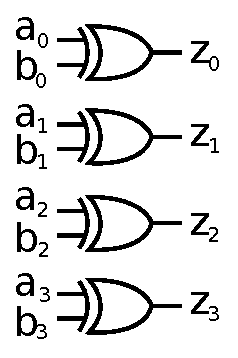
\includegraphics[scale=0.8]{figures/adder4bit.eps}
	\end{center}
	\caption{$4$-bit adder over $\mathbb{F}_{2^4}$.}
	\label{fig:adder4}
\end{figure}
\end{Example}


Conceptually, the multiplication $Z =A\times B \pmod{ P(x) }$ in $\mathbb{F}_{2^k}$ consists of two steps.
In the first step, the multiplication $A\times B$ is performed, and in the second step, the result is reduced
modulo the irreducible polynomial $P(x)$.
Multiplication procedure is shown in Example \ref{exp:mul}.

%\ref{exp1}, 
\begin{Example}
\label{exp:mul}
Consider the field $\mathbb{F}_{2^4}$. We take as inputs:
$A=a_0+a_1\cdot \alpha+a_2\cdot \alpha^2+a_3\cdot \alpha^3$ and
$B=b_0+b_1\cdot \alpha+b_2\cdot \alpha^2+b_3\cdot \alpha^3$, along
with the irreducible polynomial $P(x)=x^4+x^3+1$. We have to perform the
multiplication $Z =A\times B \pmod{ P(x) }$. The coefficients
of $A = \{a_0, \dots, a_3\}, B = \{b_0, \dots, b_3\}$ are in
$\mathbb{F}_2 = \{0, 1\}$. Multiplication can be performed as
shown below:   


{\begin{tabular}{c c c c c c c c}
  &   &   & $a_3$ & $a_2$ & $a_1$ & $a_0$  \\ 
 $\times$&   &   & $b_3$ & $b_2$ & $b_1$ & $b_0$  \\ 
 \hline
 &   &   & $a_3\cdot b_0$ & $a_2 \cdot b_0$ & $a_1\cdot b_0$ & $a_0\cdot b_0$ \\
 &  & $a_3\cdot b_1$ & $a_2\cdot b_1$ & $a_1 \cdot b_1$ & $a_0\cdot b_1$ &   \\
 & $a_3\cdot b_2$ & $a_2\cdot b_2$ & $a_1\cdot b_2$ & $a_0\cdot b_2$ &  &   \\
 $a_3\cdot b_3$ & $a_2\cdot b_3$ & $a_1\cdot b_3$ & $a_0\cdot b_3$ &  &  &   \\
 \hline
 $s_6$& $s_5$  & $s_4$  & $s_3$ & $s_2$  & $s_1$   & $s_0$ 
\end{tabular}}


The result $Sum = s_0+s_1\cdot \alpha + s_2\cdot \alpha^2 + s_3\cdot
\alpha^3 + s_4\cdot \alpha^4 + s_5\cdot \alpha^5 + s_6\cdot \alpha^6$,
\begin{eqnarray}
	s_0  &=&  a_0\cdot b_0 \nonumber \\ 
	s_1  &=&  a_0\cdot b_1 + a_1\cdot b_0 \nonumber \\
	s_2  &=&  a_0\cdot b_2 + a_1\cdot b_1 + a_2\cdot b_0 \nonumber \\
	s_3  &=&  a_0\cdot b_3 + a_1\cdot b_2 + a_2\cdot b_2 +  a_3\cdot b_1\nonumber \\
	s_4  &=&  a_1\cdot  b_3 + a_2\cdot b_1 + a_3\cdot b_1 \nonumber \\
	s_5  &=&  a_2\cdot b_3 + a_3\cdot b_2  \nonumber \\
	s_6  &=&  a_3\cdot b_3   \nonumber
\end{eqnarray}
 Here the multiply ``$\cdot$'' and add ``$+$'' operations are performed
modulo 2, so they can be implemented in a circuit using AND and XOR
gates. Note that unlike integer multipliers, there are no carry-chains
in the design, as the coefficients are always reduced modulo $p =
2$. However, the result is yet to be reduced modulo the primitive
polynomial $P(x) = x^4 + x^3 + 1$. This is shown below, where higher 
degree coefficients are reduced $\pmod{P(x)}$.
% where the final output of the circuit is denoted by $G(x)  = g_3x^3
% + g_2x^2 +g_1x + g_0$.  


{\begin{tabular}{|c c c c | l }
  $s_3$ 	&$s_2$  	&$s_1$   &$s_0$ 	&   \\
 \hline
 $s_4$ 		&$0$		&$0$ 	 &$s_4$  	&$s_4\cdot \alpha^4 \pmod{P(\alpha)} = s_4 \cdot (\alpha^3 + 1)$\\
 $s_5$ 		&$0$		&$s_5$   &$s_5$     &$s_5\cdot \alpha^5 \pmod{P(\alpha)} = s_5\cdot (\alpha^3+ \alpha + 1)$\\
 $s_6$ 		&$s_6$		&$s_6$   &$s_6$     &$s_6\cdot \alpha^6 \pmod{ P(\alpha)} = s_6\cdot( \alpha^3 + \alpha^2 + \alpha + 1)$\\
 \hline
 $z_3$ 		&$z_2$ 		&$z_1$   &$z_0$ 	&
 \end{tabular}\par}


The final result (output) of the circuit is: $Z = z_0 + z_1 \alpha + z_2
\alpha^2 + z_3 \alpha^3$; where  $z_0=s_0+s_4+s_5+s_6; ~~z_1=s_1+s_5+s_6;
~~z_2=s_2+s_6; ~~z_3=s_3+s_4+s_5+s_6$. 
\end{Example}

%%%%%%%%%%%%%%%%%%%%%%%%%%%%%%%%%%%%%%%%%%%%%%%%%%%%%%%%%%%

The above multiplier design is called the {\it Mastrovito multiplier} \cite{mastro:1989} 
which is the most straightforward way to design a multiplier over $\mathbb{F}_{2^k}$. 
A logic circuit for a $4$-bit {\it Mastrovito} multiplier over {\it finite field} $\mathbb{F}_{2^4}$ is illustrated in Fig.\ref{fig:mas4}.

\begin{figure}[b]
	\begin{center}
	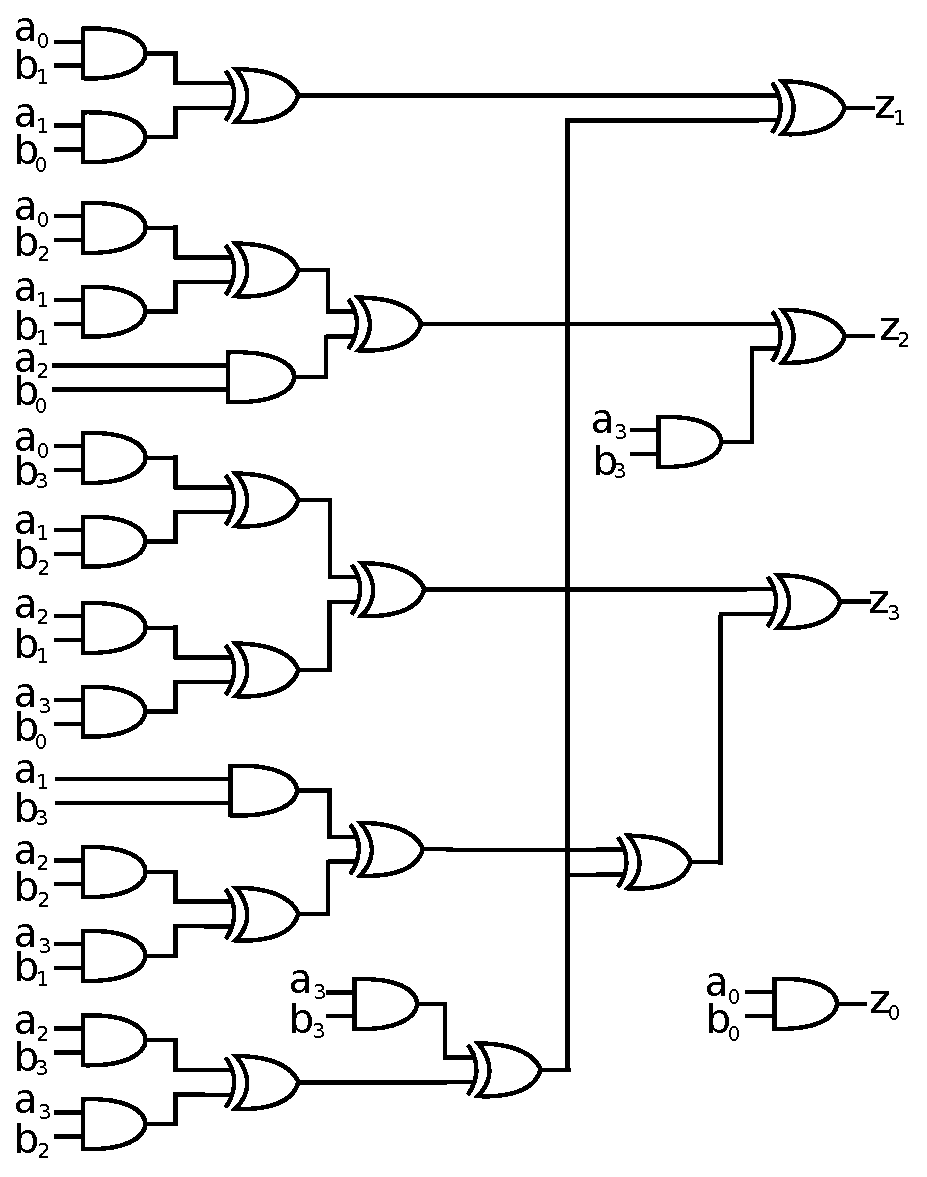
\includegraphics[scale=0.50]{figures/mul4bit.eps}
	\end{center}
	\caption{Mastrovito multiplier over $\mathbb{F}_{2^4}$.}
	\label{fig:mas4}
\end{figure}

Modular multiplication is at the heart of many public-key cryptosystems, 
such as Elliptic Curve Cryptography (ECC) \cite{ecc:1986}. 
Due to the very large field size (and hence the datapath width) used in these cryptosystems, 
the above {\it Mastrovito} multiplier architecture is inefficient, especially when exponentiation and repeat multiplications are performed.
Therefore, efficient hardware and software implementations of modular multiplication algorithms are used to overcome the complexity of such operations. 
These include the Montgomery reduction \cite{PT:1985} \cite{acar:1998} and the Barrett reduction \cite{Knezevic:2008}.

{\bf Montgomery Reduction:}  Montgomery reduction (MR) computes: 

\begin{equation}
G=MR(A,B)=A\cdot B \cdot R^{-1} \pmod {P(x)}
\end{equation}
where $A,B$ are $k$-bit inputs, $R={\alpha}^k$, $R^{-1}$ is multiplicative
inverse of $R$ in $\mathbb{F}_{2^k}$, and $P(x)$ is the irreducible polynomial for
$\mathbb{F}_{2^k}$. Since Montgomery reduction cannot directly compute $A\cdot B$, 
to compute $A\cdot B \pmod {P(x)}$, we need to pre-compute $A\cdot R$ and $B\cdot R$,
as shown in Figure \ref{fig:mm4}.  

\begin{figure}[t]
	\begin{center}
	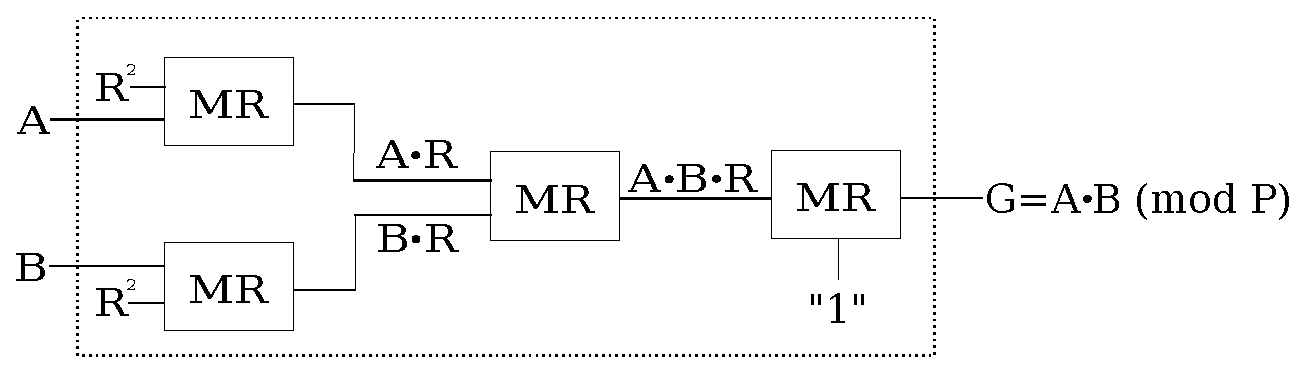
\includegraphics[scale=0.50]{figures/mmcircuit.eps}
	\end{center}
	\caption{{\it Montgomery} multiplier over $\mathbb{F}_{2^k}$}
	\label{fig:mm4}
\end{figure}

Each $\it MR$ block in Figure \ref{fig:mm4} represents a Montgomery reduction step which 
is a hardware implementation of the algorithm shown in Algorithm \ref{alg:mont}. 

\begin{algorithm}
\SetAlgoNoLine

 \KwIn{$A(x), B(x)\in \mathbb{F}_{2^k}$; irreducible polynomial $P(x)$.}
 \KwOut{$G(x)=A(x)\cdot B(x)\cdot x^{-k} \pmod {P(x)}$.}
%%%%%%%%%%%%%%%%%%%%
  $G(x):=$0 \\
  \For { ($i=0$;   $i \le k-1$; ++i ) }
  {
	$G(x):=G(x)+A_i\cdot B(x)$ \CommentSty{/*$A_{i}$ is the $i^{th}$ bit of $A$*/\;}
	$G(x):=G(x)+G_0\cdot P(x)$ \CommentSty{/*$G_{0}$ is the lowest bit of $G$*/\;}
	$G(x):=G(x) / x$ \CommentSty{/*Right shift $1$ bit*/\;}
  }
\caption{Montgomery Reduction Algorithm \cite{acar:1998}}\label{alg:mont}
\end{algorithm}

The design of Fig. \ref{fig:mm4} is an overkill to compute just
$A\cdot B \pmod{ P(x)}$. However, when these multiplications are
performed repeatedly, such as in iterative squaring, then the
Montgomery approach speeds-up the computation. 
As shown in \cite{wu:2002}, the critical path delay and gate counts of a squarer designed using the Montgomery
approach are much smaller than the traditional approaches. 


%For example, here is how to raise y to the th
%%power. I will use “*” to mean “Montgomery-multiply the numbers modulo R”
%\begin{Example}
	
%\end{Example}


{\bf Barrett Reduction:} Barrett reduction is the other widely used multiplier design method adopted in cryptography system designs.
Similar to Montgomery reduction, the traditional Barrett reduction, proposed in \cite{Barrett:1987}, needs a pre-computed value of the reciprocal/inverse of modulus $P(x)$.  
This pre-computation requires extra computational time and memory space. To overcome this limitation, the recent approach of \cite{Knezevic:2008} avoids such a pre-computation of 
inverses and therefore greatly simplifies the hardware design implementation. This algorithmic computation is shown in Algorithm \ref{alg:bar}.

\begin{algorithm}
\SetAlgoNoLine

 \KwIn{$R(x) \in \mathbb{F}_{2^k}$; irreducible polynomial $P(x)=x^n+\displaystyle\sum\limits_{i=0}^l {m_i \cdot x^i}$ satisfying $l=\lfloor \frac{n}{2} \rfloor, m_i \in \{0,1\}$.}
 \KwOut{$G(x)=R(x) \pmod {P(x)}$.}
%%%%%%%%%%%%%%%%%%%%
	$Q_1(x)=\frac{R(x)}{x^n}$ \CommentSty{/*Right shift $n$ bit*/\;}
	$Q_2(x)=P(x) \cdot Q_1(x)$ \;
	$Q_3(x)=\frac{Q_2(x)}{x^n}$ \;
	
	$G_1(x)=R(x) \pmod {x^n}$ \CommentSty{/*Keep the lower $n$ bits of $R(x)$*/\;}
	$G_2(x)=P(x)\cdot Q_3(x) \pmod {x^n}$ \;
	$G(x)=G_1(x) +G_2(x)$ \;
	
\caption{Barrett Reduction Without Pre-Computation Algorithm \cite{Knezevic:2008}}\label{alg:bar}
\end{algorithm}

Based on Barrett reduction, a multiplier can be designed with two simple steps:  multiplication $R=A \times B$ and a subsequent Barrett reduction $G=R \pmod {P}$.
This is shown in Figure \ref{fig:bar}. As we can see, a Barrett multiplier is similar to a Mastrovito multiplier except for the reduction step.

\begin{figure}[hbt]
	\begin{center}
	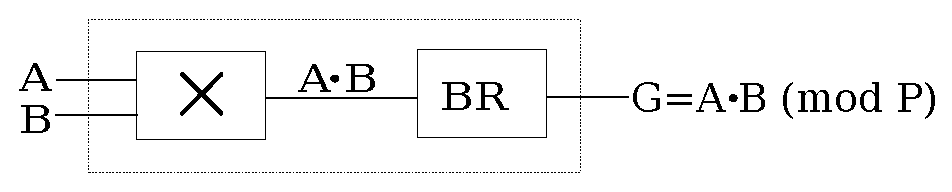
\includegraphics[scale=0.50]{figures/barrett.eps}
	\end{center}
	\caption{Barrett multiplier over $\mathbb{F}_{2^k}$.}
	\label{fig:bar}
\end{figure}

%%%%%%%%%%%%%%%%%%%%%%%%%%%%%%%%%%%%%%%%%%%
One of the most influential applications of finite fields is in elliptic curve cryptography (ECC).
ECC is an approach to public-key cryptography based on the algebraic structure of elliptic curves over finite fields.
%ECC computation is based on an elliptic curve 
The main operations of encryption, decryption and authentication in ECC rely on {\it point multiplications}.
Point multiplication involves a series of addition and doubling of points on the elliptic curve. % -- this, in turn, requires finite field multiplications. 
A drawback of traditional point multiplication is that each point addition and doubling 
involves a multiplicative inverse operation over finite fields.
Representing the points in projective coordinate systems \cite{ecc:software}
eliminates the need for multiplicative inverse operation and therefore increases the efficiency of point multiplication operation.
In our experiments, we have verified custom designs based on L$\acute{o}$pez-Dahab (LD) coordinate system \cite{eccld}. 

\begin{Example}
Consider point addition in LD projective coordinate. Given an elliptic curve: $Y^2 + XYZ = X^3Z + aX^2Z^2 + bZ^4$ over $\mathbb{F}_{2^k}$, 
where $X,Y,Z$ are $k$-bit vectors
that are elements in $\mathbb{F}_{2^k}$ and similarly, $a, b$ are constants from the field. 
Let ($X_1$, $Y_1$, $Z_1$) + ($X_2$, $Y_2$, $1$) = ($X_3$, $Y_3$, $Z_3$) represent point addition over the elliptic curve.
Then $X_3$, $Y_3$, $Z_3$ can be computed as follows:

\begin{align*}
A &= Y_2 \cdot Z_1^2 + Y_1 \\
B &= X_2 \cdot Z_1 + X_1 \\
C &= Z_1 \cdot B \\
D &= B^2 \cdot(C + a Z_1^2) \\
Z_3 &= C^2 \\
E &= A \cdot C  \\
X_3 &= A^2 + D + E  \\
F &= X_3 + X_2 \cdot Z_3 \\
G &= X_3 + Y_2\cdot Z_3 \\
Y_3 &= E\cdot F + Z_3 \cdot G \\
\end{align*}
\end{Example}

\begin{Example}
Consider point doubling in projective coordinate system. Given an elliptic curve: $Y^2 + XYZ = X^3Z + aX^2Z^2 + bZ^4$. 
Let 2($X_1$, $Y_1$, $Z_1$) = ($X_3$, $Y_3$, $Z_3$), then

\begin{align*}
X_3 &= X_1^4 + b \cdot Z_1^4  \\
Z_3 &= X_1^2 \cdot Z_1^2 \\
Y_3 &= b Z_1^4 \cdot Z_3 + X_3 \cdot (aZ_3 + Y_1^2 + bZ_1^4 ) \\
\end{align*}
\end{Example}



In the above examples, polynomoial multiplication and squaring operations are implemented 
in hardware using Montgomery or Barrett reductions over finite fields $\mathbb{F}_{2^k}$. 

The field size for such applications is generally very large; as discussed before, for ECC, in $\mathbb{F}_{2^k}$, $k=163$ or larger.  
Such large size and complicated arithmetic nature of such circuits clearly shows the complexity of the formal verification problem.
Contemporary techniques lack the requisite power of abstraction to model and verify such large systems. 
For this reason,  we propose polynomial abstractions over finite fields to model
and verify such circuits using computer algebra techniques.
This is the subject of subsequent chapters of this dissertation.

%The hardness of such designs lies in the custom-design nature of these circuits. 
%This is because finite fields arithmetic operations are computed modulo $2$, therefore there is no efficient way to describe 
%such arithmetics at high level in hardware description languages, such as {\it Verilog} or {\it VHDL}. 
%In other words, all arithmetic circuits over finite fields $\mathbb{F}_{2^k}$ have to be designed at bit level. 
%In contrast, integer arithmetics can be described easily at word level. For example, as Example \ref{exp:4bitadder}
%shows, a simple {\it Verilog} code $Result[3:0]=A[3:0]+B[3:0]$ is able to express a $4$-bit integer adder. 
%However, a $4$-bit finite field adder cannot be illustrated at word level as $Result[3:0]=A[3:0]+B[3:0]$. 
%Instead, the $4$-bit adder over finite field $\mathbb{F}_{2^4}$ requires to be designed at bit level, as shown in Example \ref{exp:ffadder}.
%Note the modulo $2$ operaton is the same as a $xor$ (\^{}) gate.

%\begin{Example}\label{exp:ffadder}
%\lstset{language=Verilog}
%\begin{lstlisting}
%module Adder(A, B, Result);

   %input [3:0] A;
   %input [3:0] B;
   %output [3:0] Result;

   %assign   Result[0] = A[0] ^ B[0];
   %assign   Result[1] = A[1] ^ B[1] ;
   %assign   Result[2] = A[2] ^ B[2];
   %assign   Result[3] = A[3] ^ B[3];
   
%endmodule
%\end{lstlisting}
%\end{Example}

%Example \ref{exp:ffadder} illustrates the difficulty of designing hardware over finite fields $\mathbb{F}_{2^k}$. 
%Accordingly, the verificaiton of such hardware is also extremely hard.
%This can be attributed to the fact that there is no efficient 
%abstract techniques available for arithmetic circuits over $\mathbb{F}_{2^k}$ 
%while such methods exist for integer arithmetic circuits.
%For example, arithmetic Bit Level (ABL) techniques can be used to abstract integer arithmetic circuits to a higher level and then conduct verification.
%However, such techniques cannot be applied for arithmetic circuits over $\mathbb{F}_{2^k}$.




